\chapter{Concept}
The application should be accessible to all employees of SinnerSchrader. Due to the heterogeneity of the people’s computer setups running Windows, macOS and Linux, creating a native application supported by everyone’s system is a rather complicated task. A web application using standard technologies does not only solve this problem, but can also be used from mobile devices such as smart phones and tablets. Furthermore, there is no need to manually install and update the software so that it can be assumed that all users use the latest version of the application. This is not only a positive factor regarding the overall usability of the system, but also assures bugs and security issues are eliminated the moment a fixed version of the software is deployed. All those advantages compared to native clients and the fact that SinnerSchrader’s expertise lies in the development of web applications lead to the decision, that such an application would be the appropriate solution.



\section{Visual Concept \& Wireframes}
The application should be as simple as possible and usable for everyone, in order to provide an efficient and fast tool. Thus, it will be designed as a single page application based around a people search that provides a way to input the skills needed and returns all persons offering said skills. After entering a search, the user can select any of the found colleagues and view their personal profile showing extended information like contact details, more skills the user did not search for, and the employee's location. This profile will also include links to directly contact the inspected person via Email or Google Hangouts(TODO: footnote). Unlike the considered commercial solutions, this tool will not include features like creating statistics, assessments, applicant management, or any dashboard other than the basic search view.
Furthermore, there will not be any different roles with different access rights for employees and their managers, since this application is meant to be a tool enhancing collaboration, not supervision.
\begin{figure}[!htp]
    \centering
    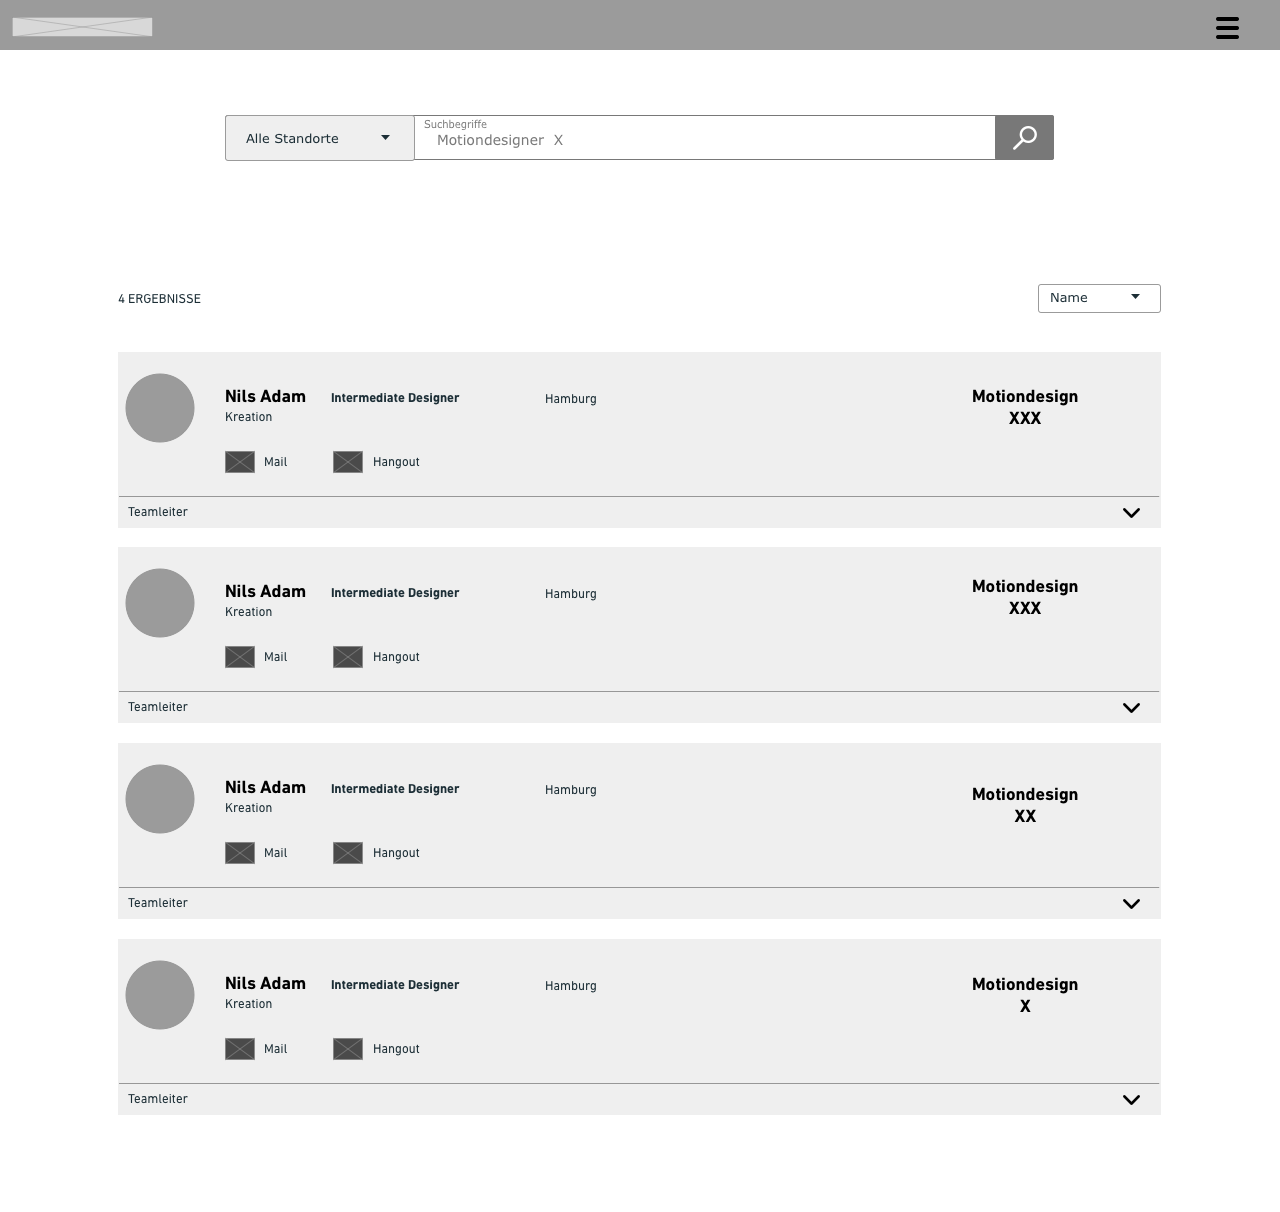
\includegraphics[width=0.8\textwidth]{images/wireframe.png}
    \caption{Wireframe}
    \label{fig:wireframe}
\end{figure}

TODO: Put UML/BPMN here



\section{Scoring Algorithm}
TODO: erklären wer was wann warum
TODO: Formel texen
